\chapter[Agent-based modelling of 3D cellular aggregates]{Agent-based modelling of 3D \\ cellular aggregates}\label{ch:2-abm}
\markboth{Agent-based modelling of 3D cellular aggregates}{}

This chapter describes the behaviour of the cellular aggregates studied in this work, and presents some simplifications to allow for its simulation. The aggregates are modelled as systems of identical spherical cells that transition from one state to another using an agent-based model.

The movement of each cell in the aggregate is governed by its equations of motion. Those depend on the interactions of each cell with nearby cells and account for friction, adhesion, and active forces. Cell differentiation is described by transition rates, which may depend on the state of the system. Our aim is to couple mechanics and cell fate transitions keeping the stochastic behaviour of both cell motion and differentiation.



\section{Proliferation}

We start from a single cell that divides into two daughter cells of the same vo\-lume, thus increasing the total volume of the aggregate over time (see Figure \ref{fig:aggregate-formation}). 

\begin{definition}
    Consider an initial cell of radius $r$, null velocity, and an arbitrary division time $t_{\text{div}}$. The rules for division for an arbitrary cell $i$ are:
    \begin{enumerate}
        \item When the simulation time $t$ exceeds the division time $t_{\text{div}_i}$, the cell divides into two identical cells positioned in opposite directions. The division axis is chosen uniformly at random and, the separation between the centres of the cells is $2r\alpha_\text{ov}$, where $0<\alpha_\text{ov}\leq1$.
        \item A new division time is assigned at random to each daughter cell using the following expression,
        $$t_{\text{div}_i} \leftarrow t + \text{U}\left(\tau_{div}(1-\sigma_{div}),\tau_{div}(1+\sigma_{div})\right),$$
        where $\text{U}(a,b)$ denotes the uniform distribution. Both daughter cells are initialized at half of the velocity of the mother cell before division in order to enforce momentum conservation.
    \end{enumerate}
\end{definition}

\begin{figure}[h]
    \centering
    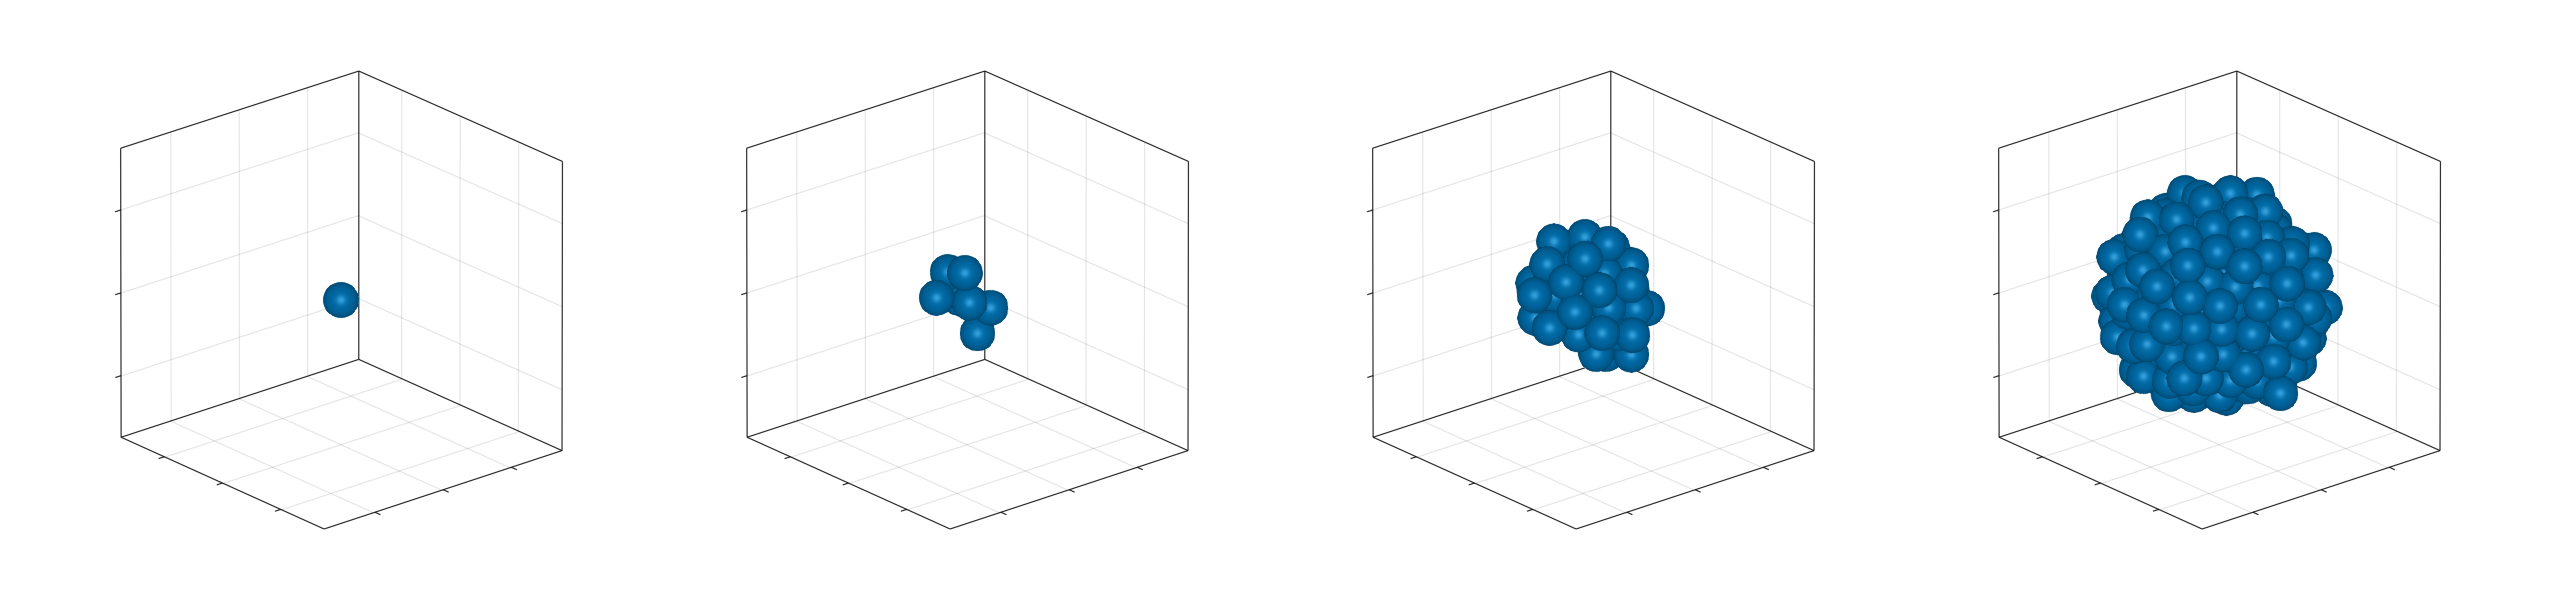
\includegraphics[width=\textwidth]{figures/400/400-aggregate-formation.png}
    \caption{Formation of a 300-cell multicellular aggregate.}
    \label{fig:aggregate-formation}
\end{figure}



\section{Mechanical interactions}

\subsection{The equations of motion}

Cells exert and receive forces that condition their movement and organization in the aggregate. Next, we define the equations of motion of each cell, considering friction forces, passive forces, and active forces \parencite{Liedekerke_2015}. Let us define the system and break down every component.

\begin{definition}
    Each cell $i$ behaves according to the following equations of motion,
    \begin{align}
        \begin{aligned}\label{eq:og_motion}
            m\frac{\diff v_i}{\diff t} &=-\Lambda\sum_{j\in U_i}(v_i-v_j)+
            \sum_{j=1}^{N} F_{ij} + F_{a_i}\\
            \frac{\diff x_i}{\diff t} &=v_i,
        \end{aligned}
    \end{align}
    with initial conditions
    \begin{equation}
        v_i(0) = v_{0_i} \qquad x_i(0) = x_{0_i},
    \end{equation}
    where $x,v\in\R^3$ represent the position of the centre and the velocity, respectively. Here, $\Lambda$ is the friction coefficient, and $U_i$ denotes the set of neighbouring cells.
\end{definition}

\begin{definition}
    Two cells $i$ and $j$ are said to be neighbours if and only if 
    $$d_{ij}<2\alpha_\text{nb} r,$$ 
    where $\alpha_\text{nb}\in\R$ is the neighbouring range, and $d_{ij} = |x_i-x_j|$ is the Euclidean distance in $\R^{3}$ between cells $i$ and $j$. The set of neighbours (or neighbourhood) of cell $i$ is defined as
    $$U_i=\{j:d_{ij}<2\alpha_\text{nb}\},$$
    and $n_i=|U_i|$ denotes the number of neighbours of cell $i$.
\end{definition}

\begin{notation}
    Variables regarding the agents change over time. Notation such as $U_i$ and $d_{ij}$ refers to the time-dependent functions $U_i(t)$ and $d_{ij}(t)$.
\end{notation}

The first term in the right-hand side of Equation \ref{eq:og_motion} represents the friction forces. These forces are dependent on the relative velocity of the cell with res\-pect to its neighbours. The last two terms correspond to passive and active forces, respectively. Active forces can be due to processes such as filopodia bet\-ween cells, and will be described later in this section.

Passive forces exerted by nearby cells are modelled as piecewise functions with repulsive and attractive regimes, which take into account steric interactions and cell-cell adhesion, respectively \parencite{Saiz_2020,Torregrosa_2023}.

\begin{notation}
    The range of cells that forces take into account is slightly larger than the neighbouring range. These are referred to as {nearby cells} throughout the text to distinguish them from neighbouring cells.
\end{notation}

\begin{definition}
    The passive force $F_{ij}\in\R^3$ exerted by cell $j$ over cell $i$ is given by
    \begin{equation}\label{eq:fij}
        F_{ij}=
        \begin{dcases}
            \frac{(x_i-x_j)}{d_{ij}} 
            F_0 f_r(d_{ij})\alpha_\text{adh}\alpha_\text{rep}
            &\quad \text{if $d_{ij}\leq 2 r$} \\
            \frac{(x_i-x_j)}{d_{ij}}
            F_0 f_r(d_{ij}) \alpha_\text{adh}
            &\quad \text{if $2r<d_{ij}<2\mu r$} \\
            0 &\quad \text{otherwise,}
        \end{dcases}
    \end{equation}
    where $\mu>0$ is the force range factor, and  $\alpha_\text{adh}, \alpha_\text{rep}>0$ are the adhesion and repulsion factors, respectively. Here, $F_0>0$ denotes the typical force generated by cells, and
    \begin{equation}
        f_r (d_{ij})=
        \left(\frac{2r}{d_{ij}}-1\right)
        \left(\frac{2\mu r}{d_{ij}}-1\right)
        \in\R.
    \end{equation}
\end{definition}

The reasoning behind this expression is discussed in Section \ref{sec:avg_nbs}.

\begin{remark}
    The adhesion factor accounts for differences in the adhesion strength for each pair. Unless stated otherwise, it is assumed to be $\alpha_\text{adh}\equiv 1$.
\end{remark}

The function $f_r$ determines whether the force is attractive ($f_r<0$) or repulsive ($f_r>0$). When there exists an overlap between cells, e.g. after the two daughter cells are created, cells are pushed away from each other until their distance reaches the equilibrium distance $2r$. 

\begin{remark}\label{rk:regimes}
    The behaviour of the force depends on the distance as follows.
    \begin{itemize}
        \item If $d_{ij} < 2r$, then $f_r>0$. The force is repulsive when the cells are separated below their equilibrium distance.
        \item If $d_{ij}=2r$, then $f_r=0$. There is no force when the separation is exactly the equilibrium distance.
        \item If $2r<d_{ij}<2\mu r$, then $f_r<0$. The force is attractive when the cells are separated slightly above the equilibrium distance.
        \item If $2\mu r \leq d_{ij}$, then $f_r=0$. There is no force when the cells are far apart.
    \end{itemize}
\end{remark}

A sketch of the $f_r$ function is shown in Figure \ref{fig:force_function}.

\begin{figure}[htp] % Positioning options: h = here, t = top, b = bottom, p = page
    \centering
    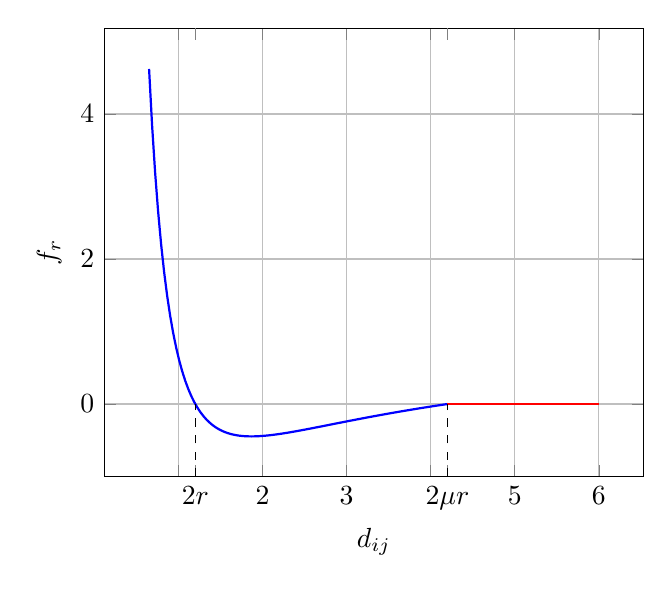
\begin{tikzpicture}
        \begin{axis}[
            xlabel={$d_{ij}$}, 
            ylabel={$f_r$},
            % title={title}
            grid=both,
            domain=0:6,
            samples=100, 
            ymin=-1,
            xtick={1, 2, 3, 4, 5, 6},
            xticklabels={,2,3,,5,6}, 
            extra x ticks={1.2, 4.2}, 
            extra x tick labels={$2r$, $2\mu r$},
            extra x tick style={grid=none}
        ]
            \addplot[domain=0.65:4.2, samples=100, thick, color=blue] {(2*0.6/x - 1)*(2*.6*3.5/x - 1)};
            \addplot[domain=4.2:6, samples=100, thick, color=red] {0};

            \addplot[dashed, thin, black] coordinates {(1.2, -1) (1.2, 0)};
            \addplot[dashed, thin, black] coordinates {(4.2, -1) (4.2, 0)};
            
        \end{axis}
    \end{tikzpicture}    
    \caption{Example plot of the function $f_r$ for $r=0.6$, $\mu=3.5$.}
    \label{fig:force_function}
\end{figure}


\subsection{Accounting for random cell-cell interactions}

Cells exhibit subtle displacements caused by active forces, causing a continuous reorganization of the aggregate. We model such forces to mimic the behaviour of filopodia, dynamic structures that extend from the cell membrane and connect to nearby cells. These cell-cell interactions result in temporal directed pairwise forces, which we refer to as protrusions \parencite{Oriola_2022,Torregrosa_2023}.

\begin{definition}
    Each cell has an associated protrusion function $P_i\in\{0,1,-1\}$ such that $P_i=0$ if the protrusion is inactive. Protrusions are modelled according to the following rules:
    \begin{enumerate}
        \item The probability of activating an inactive protrusion after a time $\Delta t$ is $k_{p_\text{on}}\Delta t$, where $k_{p_\text{on}}$ is the protrusion activation rate.
        \item If $P_i$ is activated at the previous step, set $P_{i}=1$.
        \begin{enumerate}[label=\roman*.] % [label=\theenumi.\arabic*.]
            \item Choose a random inactive nearby cell $j$ is and set $P_j=-1$.
            \item Choose a random number $\xi\sim \text{U}(0,1)$.
            \item Let $k_{p_\text{off}}$ be the protrusion deactivation rate. Set a random protrusion time $t_{ij}$ to both $i$ and $j$,
                $$t_{ij} \leftarrow t - \frac{\log(\xi)}{k_{p_\text{off}}}.$$
        \end{enumerate}
        \item While $t<t_{ij}$, cell $i$ exerts a protrusion force $F_{p_i}\in\R^3$ on cell $j$.
        \item When $t\geq t_{ij}$, then $P_i=P_j=0$ and the cells become again eligible to be connected with another random inactive cell.
    \end{enumerate} 
\end{definition}

\begin{definition}
    Let $D>0$ be the protrusion strength constant. The protrusion force is given by
    \begin{equation}\label{eq:fp}
        F_{p_i}=
        \begin{dcases}
            - \frac{(x_i-x_j)}{d_{ij}} D \alpha_\text{rep}
            &\quad \text{if $d_{ij}\leq 2 r$} \\
            - \frac{(x_i-x_j)}{d_{ij}} D
            &\quad \text{if $2r<d_{ij}<2\mu r$},
        \end{dcases}
    \end{equation}
    and $|F_{p_i}|\in\{D \alpha_\text{rep},D\}$.
\end{definition}

\begin{remark}
    Modelling the active forces as the protrusion force, Equation \ref{eq:og_motion} becomes
    \begin{align}\label{eq:moton_fp}
        \begin{aligned}
            m\frac{\diff v_i}{\diff t} &=-\Lambda\sum_{j\in U_i}(v_i-v_j)+
            \sum_{j=1}^{N} F_{ij} + P_i F_{p_i}\\
            \frac{\diff x_i}{\diff t} &=v_i,
        \end{aligned}
    \end{align}
    where $P_i F_{p_i}\in\{-F_{p_i},F_{p_i},0\}.$
\end{remark}


\subsection{Simplification of the mechanics}\label{sec:simplify}

Next, we simplify the equations of motion that govern the model. In the context of cell movement in cellular tissues, viscous forces dominate over inertial forces; thus, the system is assumed to be in the overdamped regime \parencite{Purcell_1977,Liedekerke_2015}. 

Under these circumstances, the inertia term $m\frac{\diff v_i}{\diff t}$ is negligible, and thus the previous equation becomes
\begin{equation}\label{eq:overdamped}
    0 =-\Lambda\sum_{j\in U_i}(v_i-v_j)+
    \sum_{j=1}^{N} F_{ij} + P_i F_{p_i}.
\end{equation}

In 2D cell monolayers, the friction force originates from the interaction between the cell and the substrate, and is proportional to the velocity of the cell. However, in 3D aggregates the friction force is proportional to the relative velocities between cells \parencite{Liedekerke_2015}, as stated in Equation \ref{eq:overdamped}. Still, we will show that, performing the appropriate approximations, one can simplify the friction term to $\Lambda v_i$.

In Ya||a \parencite{Germann_2019}, a CUDA/C++ agent-based model, the friction term in Equation \ref{eq:overdamped} is simplified as follows,
\begin{equation}
    -n_i \Lambda \left(v_i - \frac{1}{n_i}\sum_{j\in U_i}v_j\right)
    \approx -\lambda \left(v_i - \frac{1}{n_i}\sum_{j\in U_i}v_j\right),
\end{equation}
approximating the time dependent friction coefficient $n_i\Lambda$ by a global coefficient $\lambda$. 

This estimate only approximates $n_i$ in one of its two instances. Next, we propose an alternative approach. In Section \ref{sec:avg_nbs}, we test computationally the two assumptions that will be presented, and discuss possible issues. 

First, we rewrite Equation \ref{eq:overdamped} as follows,
\begin{equation}
    \Lambda n_i v_i =\Lambda\sum_{j\in U_i}v_j+\sum_{j=1}^{N} F_{ij} + P_i F_{p_i}.
\end{equation}

In the absence of net flows in the tissue, we can perform the following approximation,
\begin{equation}\label{eq:netflows}
    \sum_{j\in U_i}v_j\approx 0.
\end{equation}

Finally, we take the average number of neighbours to be constant over time, and approximate the friction term by a global friction term $\lambda$ for all cells and time,
\begin{equation}\label{eq:globalfriction}
    \Lambda n_i(t) \approx \lambda>0.
\end{equation}

\begin{proposition}
    Applying the simplifications presented in this section, the equations of motion become
    \begin{align}\label{eq:motion_dim}
        \begin{aligned}
            \lambda v_i &= \sum_{j=1}^{N} F_{ij} + P_i F_{p_i}\\
            \frac{\diff x_i}{\diff t} &=v_i.
        \end{aligned}
    \end{align}
\end{proposition}



\section{Cell differentiation}\label{sec:diff}

During animal development, stem cells differentiate and give rise to all the different cell types in the organism. Over time, their protein composition and gene expression profile change irreversibly. The time evolution of a cell can be split in states: we say that a cells transition to a new state (or cell fate) when their gene expression profile has changed significantly such that it can be considered a different type of cell.

This coarse-grained approach greatly simplifies the analysis: instead of studying the continuous changes in the composition of cells, it is enough to study the discrete dynamics of cell transitions. We will use a unidirectional stochastic process for differentiation, where the transition rates may change depending on the spatial organization of the aggregate. 

First, we need some preliminary definitions. Let $X$ denote an arbitrary cellular state.

\begin{definition}
    The transition rate $r_{X\rightarrow Y}^{(i)}(t)$ describes the probability per unit time of a cell in state $X$ to transition to state $Y$.
\end{definition}

\begin{definition}
    Let $\text{state}(i)$ denote the state of cell $i$. The state indicator function for cell $i$ is
    \begin{align}
        \mathds{1}_X(i)&=\begin{cases}
            1\quad\text{if }\text{state}(i)=X\\
            0\quad\text{otherwise}.
        \end{cases}
    \end{align}
\end{definition}

\begin{definition}
    The proportion of cells in state $X$ is denoted as follows,
    \begin{align}
        \phi_X&=\frac{1}{N}\sum_{i}^{N}{\mathds{1}_X(i)}.
    \end{align} 
\end{definition}

\begin{remark}
    The sum of the proportions is always one, that is,
    \begin{align*}
        \phi_A + \phi_B + \phi_C = 1.
    \end{align*}
\end{remark}

\begin{definition}\label{def:prop_ngb}
    The proportion of neighbours of cell $i$ in state $X$ is denoted as follows,
    \begin{align}
        \langle\mathds{1}_X(i)\rangle&=\frac{1}{n_i}\sum_{j\in U_i}{\mathds{1}_X(i)}.
    \end{align} 
\end{definition}

In this work we consider three possible states: $A$, $B$ and $C$. Once the differentiation process begins, cells start transitioning with certain rates from its initial state $A$ to state $B$, and from state $B$ to state $C$. Next, we describe three different expressions for the transition rates. The physical effect of these expressions is compared in Chapter \ref{ch:4-applications}.

\begin{definition}
    Let the transition rates be independent of the cell,
    \begin{equation*}
        r_{X\rightarrow Y}^{(i)}(t)\equiv r_{X\rightarrow Y}(t).
    \end{equation*}
    Then, the evolution of the state proportions is described by the following system of differential equations,
    \begin{equation}\label{eq:proportions}
        \begin{aligned}
            \dot\phi_A&=-r_{A\rightarrow B}\phi_A \\
            \dot\phi_B&=r_{A\rightarrow B}\phi_A - r_{B\rightarrow C}\phi_B  \\
            \dot\phi_C&=r_{B\rightarrow C}\phi_B,
        \end{aligned}
    \end{equation}
    with initial conditions
    \begin{equation}
        \begin{aligned}
            \phi_A(0) &= a\\
            \phi_B(0) &= 1-a\\
            \phi_C(0) &= 0.
        \end{aligned}
    \end{equation}
\end{definition}



\subsection{Linear first order differentiation kinetics}

The simplest scenario is to consider that cells differentiate with a constant rate, independently of the state of their surrounding cells.

\begin{definition}\label{def:constant-rates}
    When the transition rates are constant, we denote them by
    \begin{align}
        \begin{aligned}
            r_{A\rightarrow B} &= p\\
            r_{B\rightarrow C} &= q.
        \end{aligned}
    \end{align}
\end{definition}

In this case, Equation \ref{eq:proportions} can be easily solved analytically. The advantage of studying simpler cases first is that they are easier to simulate, and their solution allow us to check if the simulations work accurately.

\begin{proposition}\label{prop:analytical}
    When the transition rates are constant, we can compute the analytical solution of Equation \ref{eq:proportions}.
\end{proposition}

The expression for the analytical solution and the proof of Proposition \ref{prop:analytical} are detalied in Section \ref{sec:derivations} of the Appendix.

However, cells usually communicate through morphogenetic signals which induce cell differentiation. Next, we consider such a case.


\subsection{Nonlinear differentiation kinetics}

In this case, transition rates are no longer constant and change over time depending on the surrounding cells. The origin of these nonlinearities is the consequence of feedback in the transition rates.

\begin{definition}
    There is feedback in the transition from one state to another when the transition rate depends on the state of the rest of cells. The feedback factor $K\geq0$ determines the strength of this process.
\end{definition}

In particular, we consider the case in which the rates $r_{A\rightarrow B}$ and $r_{B\rightarrow C}$ depend on the proportion of cells in state $A$ following two different approaches. This choice is motivated by experimental evidence in mouse gastruloids \parencite{Oriola_2025}. For $K=0$, we recover the linear first order kinetics.

Next, we consider a mean field model for feedback. This model assumes that the transition rate of a cell is affected by the global state of the aggregate.

\begin{definition}
    Using mean field feedback, the transition rates depend on the total proportion of cells in state $A$,
    \begin{align}\label{eq:rates-mf}
        \begin{aligned}
            r_{A\rightarrow B}&=\frac{p}{1+K\phi_A}\\
            r_{B\rightarrow C}&=\frac{q}{1+K\phi_A}.
        \end{aligned}
    \end{align}
\end{definition}
Note that, in this case, the transition rates at each time are equal for all cells. Therefore, we can solve Equation \ref{eq:proportions} numerically.

The third approach implies paracrine signalling, that is, cell-cell signalling that induces changes in neighbouring cells.  Intuitively, if $A$ cells are evenly distributed across the aggregate, this will be similar to Equation \ref{eq:rates-mf} for all cells. 

\begin{definition}
    Using cell-cell signalling feedback, the transition rates depend on the proportion neighbours in state $A$,
    \begin{align}
        \begin{aligned}
            r_{A\rightarrow B}^{(i)}&=\frac{p}{1+K\langle\mathds{1}_A(i)\rangle}\\
            r_{B\rightarrow C}^{(i)}&=\frac{q}{1+K\langle\mathds{1}_A(i)\rangle}.
        \end{aligned}
    \end{align}
\end{definition}

Usually, cell states are not evenly mixed across the aggregate, so this method mirrors the experimental results more accurately. However, it is not possible to describe a numerically solvable system. The simulation presented in this thesis integrates cell-cell signalling feedback and offers a solution to the evolution of the proportions of each state over time (see Chapter \ref{ch:4-applications}). 

Making sure that the model simulates the previous differentiation kinetics according to the known solutions will be crucial to confidently implement cell-cell feedback.



\section{Nondimensionalization}\label{sec:nondimensionalization}

Nondimensionalization is a process used to remove the units from variables. It involves scaling the variables in a system by appropriate factors.

\begin{definition}
    The reference values used to scale each variable are
    $$(F_0,R_0,T_0).$$
\end{definition}

\begin{notation}
    Dimensionless variables are denoted by a tilde $\sim$.
\end{notation}

\begin{example}
    Let $[F],{[T]},{[L]}$ be the units of force, time, and length respectively. The, the units of friction $\lambda$ are $\frac{[F][T]}{[L]}$, and it is nondimensionalized w.r.t. the reference values as
    $$\tilde \lambda\equiv \lambda\frac{1}{F_0}\frac{R_0}{T_0}.$$
\end{example}

Following this process, the dimensionless variables of the model are
\begin{equation}
    \tilde F \equiv \frac{F}{F_0},
    \qquad \tilde t \equiv \frac{t}{T_0},
    \qquad \tilde r_{X\rightarrow Y} \equiv {T_0}r_{X\rightarrow Y},
\end{equation}
and
\begin{equation}
    \qquad \tilde x \equiv \frac{x}{R_0},
    \qquad \tilde v \equiv v\frac{T_0}{R_0},
    \qquad \tilde \lambda\equiv \lambda\frac{R_0}{F_0T_0}.
\end{equation}

\begin{proposition}\label{prop:nondim}
    The dimensionless equations of motion are
    \begin{align}
        \begin{aligned}\label{eq:motion}
            \tilde \lambda \tilde v_i &=\sum_{j=1}^{N}\tilde F_{ij} + P_k \tilde F_{p_i}\\
            \frac{\diff \tilde x_i}{\diff\tilde t} &=\tilde v_i,
        \end{aligned}
    \end{align}
    with initial conditions
    \begin{equation}\label{eq:motion-ic}
        \tilde v_i(0) = \tilde v_{0_i}, \qquad \tilde x_i(0) = \tilde x_{0_i}.
    \end{equation}
\end{proposition}

\begin{proof}
    The proof of Proposition \ref{prop:nondim} is derived in Section \ref{sec:derivations} of the Appendix.
\end{proof}

These are the final equations used to simulate the motion of the cells in the aggregate.
